\documentclass[11pt, a4]{article}
\usepackage[a4paper, top=1in, bottom=1in, left=1in, right=1in]{geometry}
\usepackage{color} 
\usepackage[pdftex]{hyperref}
\hypersetup{colorlinks=true, linktoc=all, linkcolor=black,}
\usepackage[export]{adjustbox}
\usepackage{float}
\restylefloat{table}
\usepackage{array}
\usepackage[activate={true,nocompatibility},final,tracking=true,kerning=true,spacing=true,factor=1100,stretch=10,shrink=10]{microtype}
\usepackage{tikz}
\usepackage{graphicx}
\usepackage{pgfplots}
\pgfplotsset{scaled y ticks=false}
\usepackage{multirow}
\usepackage{callouts}
\usepackage{mhchem}
\usepackage{longtable}
\usepackage{array}
\usepackage[justification=centering]{caption} 
\usepackage{titlesec}
\usepackage{amsmath}
\usepackage{amssymb}
\usepackage{circuitikz}
\usepackage[font=small, skip=0pt]{caption}

\title{\vspace{90mm}Investigating the effect of changes in potential difference on the electrolysis of 1M Copper(II) Sulphate ($ CuSO_{4} $) with the utilisation of copper electrodes} 
\author{Adithya Narayanan}
\date{18 November, 2019}

\begin{document}
	\begin{titlepage}
		\maketitle
		\thispagestyle{empty}
	\end{titlepage}
	\tableofcontents
	\thispagestyle{empty}
	\newpage
	\clearpage
	\setcounter{page}{1}
	\section{Aim:}
		\subsection{Research question:}
			To investigate the relationship and effect of changes in the potential difference (as a quantitative method of manipulating current) on the loss of mass at the anode (as a quantitative measure for the rate of reaction) in an electrolysis reaction of Copper(II) Sulphate (CuSo$_{4}$), which will be achieved by changing the potential difference given to the circuit at the source for and performing a total of 18 electrolysis Oxidation-Reduction (Redox) reactions with 6 different potential difference values of 2, 4, 6, 8, 10 and 12 Volts (V) for a total of 6 datasets, each with 3 trials, while measuring the loss in mass at the anode by measuring the original mass of the anode prior to and following the electrolysis reaction and utilising these values in to calculate the loss in mass at the anode. The data collected will help show the effect that different potential difference values, used to manipulate current, have on the reaction rate of the electrolysis setup, which can be observed through the loss in mass at the anode in 4 minutes for each trial.
			
		\subsection{Background information:}
			Electrolysis is an electrochemical redox (portmanteau of Reduction-Oxidation) reaction utilised to decompose an ionic compound into its constituent ions, by passing an electrical current through the electrolytic form of the compound. In order to conduct electrolysis, the compound is first melted into its liquid state or dissolved into a solvent such as water, thus constituting the electrolyte. The electrostatic attraction between the ions of the compound remains inversely proportional to the relative permittivity of the surrounding medium, given by the equation for Coulomb's law (all units in SI units):
			
			\begin{equation}
				F_{e} = k \frac{q_{1}q_{2}}{r^{2}}
			\end{equation}
				
				where $q_{1}$ and $q_{2}$ represent the magnitude of the 2 charges, $r^{2}$ represents the distance between the 2 charges and k represents the Coulomb's constant of the specific medium, calculated using the following equation:
				
			\begin{equation}
				k = \frac{1}{4 \pi \epsilon}
			\end{equation}
			
			where $\epsilon$ represents permittivity of the medium. The permittivity of the medium can be calculated using the following equation:
			
			\begin{equation}
				\epsilon = \epsilon _{r}\epsilon_{0}
			\end{equation}
			
			where $\epsilon _{r}$ represents the relative permittivity and $\epsilon _{0}$ represents permittivity in a vacuum, set to be 1.
			
			\bigbreak
			
			Given that the relative permittivity ($\epsilon _{r}$) of water is around 80.2 at 20$^{o}C$ (due to the electronegativity of the Oxygen ions in water), it can be observed that the Coulomb's constant for water is calculated to be:
			
			\begin{equation*}
				k = \frac{1}{320.8\pi}
			\end{equation*}
			
			It can be observed from the value for relative permittivity, water maintains a great tendency to distort electric fields. Substituting this value into Coulomb's law gives:
			
			\begin{equation*}
				F_{e} = \frac{q_{1}q_{2}}{320.8 \pi r^{2}}
			\end{equation*}

			
			Thus, it can be observed that the coulomb's force between the ions of the compound decreases significantly when dissolved in water, assuming all other variables remain constant. Hence, the compound dissociates into its constituent free anions and cations. It can be observed that the dissolution of the compound allows for the free movement of ions and therefore, allows electricity to flow freely through the liquid, thus being considered an electrolyte.
			 
			\bigbreak
			
			Following this, 2 electrodes are partly immersed in the electrolyte and are connected to a power source providing direct current (D.C), to create a potential difference. With a closed loop now being created, when an electrical current is passed through the circuit, the free moving negatively charged anions are attracted to the anode (electrode connected to the positive terminal), and the positively charged cations are attracted to the cathode (electrode connected to the negative terminal), following Coulomb's law \footnote{Like charges repel; unlike charges attract}. At the anode, anions lose electrons from their valence shell, with the inverse occurring at the cathode.
			
			\bigbreak
			
			In the case of an aqueous solution, Hydroxyl radicals (OH$^{-}$) and non-metal ions are attracted to the anode. The more reactive ion remains in solution and the less reactive ion loses electrons more readily and is thus discharged from the solution. However, this may vary depending on the electrode used and other factors such as the concentration of the solution. For example, the more concentrated ion present in solution is more likely to discharged at the anode, than the more dilute ion. 
			
			\bigbreak
			
			The remaining hydrogen (H$^{+}$) and metal ions are attracted to the cathode. In this case, either hydrogen or the metal ion is discharged, depending on the metal's position in the reactivity series. If the metal is below hydrogen, the metal ions are discharged or precipitate from the solution onto the electrode. However, if the metal is above hydrogen, hydrogen gas is produced instead.
			
			\bigbreak
			
			The number of moles (mol) of the respective product liberated at an electrode can be calculated using the following equation:
			
			\begin{equation}
				n \ (mol) \ = \ \frac{Q \ (C)}{zF}
			\end{equation}
			
			where $Q$ represents charge in Coulombs (C), $z$ represents the charge number of the liberated ion, and $F$ represents Faraday's constant, approximately $96485.332 C/mol$. The equation for charge:
			
			\begin{equation}
				Q \ (C) \ = \ I \ (A) \ \Delta t \ (s)
			\end{equation}
			
			where I represents current in Amperes (A) and t represents time in Seconds (s), can be substituted into the original equation to give:
			
			\begin{equation}
				n \ (mol) \ = \ \frac{I \ (A) \ \Delta t \ (s)}{zF}
			\end{equation}
			
			\subsubsection{Theory:}
				In the case of aqueous $Copper(II) \ Sulphate$, the $CuSO_{4}$ molecules dissociate into $Cu^{2+}$ and $SO_{4}^{2-}$ free cations and anions respectively when dissolved. The $Cu^{2+}$ and $H^{+}$ ions are attracted to the cathode and the $SO_{4}^{2-}$ and $OH^{-}$ ions are attracted to the anode. Upon approaching the cathode, the $Cu^{2+}$ ions gain 2 valence shell electrons to become elemental copper atoms and precipitate onto the cathode, giving the following reduction half equation:
				
				\begin{equation}
					\ce{Cu^{2+}_{(aq)} + 2e^{-} -> Cu_{(s)}}
				\end{equation}
				
				The $H^{+}$ ions remain in solution as Copper is below Hydrogen in the reactivity series and is discharged preferentially.
				
				\bigbreak
				
				On the other hand, as the $SO_{4}^{2-}$ radical cannot exist in an electrically neutral state, and as Copper is more electronegative than both the $OH^{-}$ ions and the $SO_{4}^{2-}$ ions, the elemental copper atoms at the anode begin preferentially losing valence shell electrons to become $Cu^{2+}$ ions, giving the following oxidation half equation:
				
				\begin{equation}
					\ce{Cu_{(s)} -> Cu^{2+}_{(aq)} + 2e^{-}}
				\end{equation}
				
				The $SO_{4}^{2-}$ ions attempt to reform $CuSO_{4}$ molecules with the $Cu^{2+}$ ions, however cannot due to the high relative permittivity of water (refer to equation 1), hence they remain as free anions and cations. The $Cu^{2+}$ ions are once again attracted to the cathode and the $SO_{4}^{2-}$ ions become attracted to the anode and the process repeats, causing the anode to erode and lose mass while the cathode gains mass. For every copper ion reduced, one copper atom is oxidised from the anode, hence it can be deduced that the loss in mass at the anode is equivalent to the gain in mass at the cathode, assuming the electrodes are composed of pure copper. The solution remains relatively blue, as $CuSO_{4}$ ions discharged at the cathode are constantly being replaced by $CuSO_{4}$ ions oxidised at the anode.
			
			\bigbreak
			
			In the case of Ohmic conductors such as a wire, an increase in the potential difference would cause a direct increase in the current flowing through the wire. When applying this concept to the case of electrolysis, the increase in the current flowing through the circuit would cause an increase in the physical number of electrons passing from one electrode to another. This increases the rate of the electrochemical reaction and hence the anode will erode faster and the cathode will gain mass faster. The direct effect of potential difference on the rate of the reaction allows for manipulations of the potential difference to provide quantitative changes in the data collected.
			
			\subsection{Predicted data and graphical outcome:}
				\subsubsection{Predicted data:}
					\begin{table}[H]
				\begin{minipage}{\textwidth}
					\begin{adjustbox}{width= \textwidth, center=\textwidth}
						\centering
						\begin{tabular}{|>{\centering\arraybackslash}p{4.45cm}|>{\centering\arraybackslash}p{4.45cm}|>{\centering\arraybackslash}p{6.9cm}|}
							\hline
							\multicolumn{3}{|>{\centering\arraybackslash}p{15.9cm}|}{\textbf{Predicted data table for average loss in mass at anode (mol) in 4 minutes for various potential difference (V) values in the electrolysis of CuSO$_{4}$ using copper electrodes}}\\
							\hline
							\textbf{Potential difference (V)} & \textbf{Current passing through electrolyte (A)} & \textbf{Predicted average loss in mass at anode (mol, 6 d.p)}\\
							\hline
							\hline
							2 & 0.3 & 0.000373\\
							\hline
							4 & 0.6 & 0.000746\\
							\hline
							6 & 0.9 & 0.001119\\
							\hline
							8 & 1.2 & 0.001492\\
							\hline
							10 & 1.5 & 0.001866\\
							\hline
							12 & 1.8 & 0.002239\\
							\hline
						\end{tabular}
					\end{adjustbox}
				\end{minipage}
			\end{table}
			
			Above is a table of predicted data for the loss in mass at the electrode calculated using equation 6 for various potential difference values. The current readings for different potential difference values were recorded during trial runs and were utilised to predict the above data.
			
				\subsubsection{Sample calculations:}
					\textbf{Sample calculation for the predicted loss in mass at a potential difference of 2 V:}
					\begin{equation*}
						\begin{split}
							n &= \frac{0.3 \ A \times 240 \ s}{2 \times 96485.332 \ C/mol}\\
							&= \frac{72 \ C}{192970.664 \ C/mol}\\
							&= 0.000373 \ mol \ (6 d.p)\\
						\end{split}
					\end{equation*}
				$\therefore$ the predicted loss in mass at the anode is 0.000373 mol (6 d.p) at a potential difference of 2V.
				
				\subsubsection{Graphical outcome:}
				\begin{figure}[H]
					\vspace{-4mm}
					\begin{center}
					\pgfplotsset{width=13cm,
					node near coord/.style args={#1/#2/#3}{% Style for activating the label for a single coordinate
						nodes near coords*={
							\ifnum\coordindex=#1 #2\fi
						},
						scatter/@pre marker code/.append code={
							\ifnum\coordindex=#1 \pgfplotsset{every node near coord/.append style=#3}\fi
						}
					},
					nodes near some coords/.style={ % Style for activating the label for a list of coordinates
						scatter/@pre marker code/.code={},% Reset the default scatter style, so we don't get coloured markers
						scatter/@post marker code/.code={},% 
						node near coord/.list={#1} % Run "node near coord" once for every element in the list
					}
				}
				\pgfplotstableread{
					V M
					2 0.000373
					4 0.000746
					6 0.001119
					8 0.001492
					10 0.001866
					12 0.002239
				}\datatablepredicted
				
				\pgfplotstableread{
					V M
					2 0.000361
					4 0.000604
					6 0.000906
					8 0.001534
					10 0.001901
					12 0.002548
				}\datatablefinal
				
					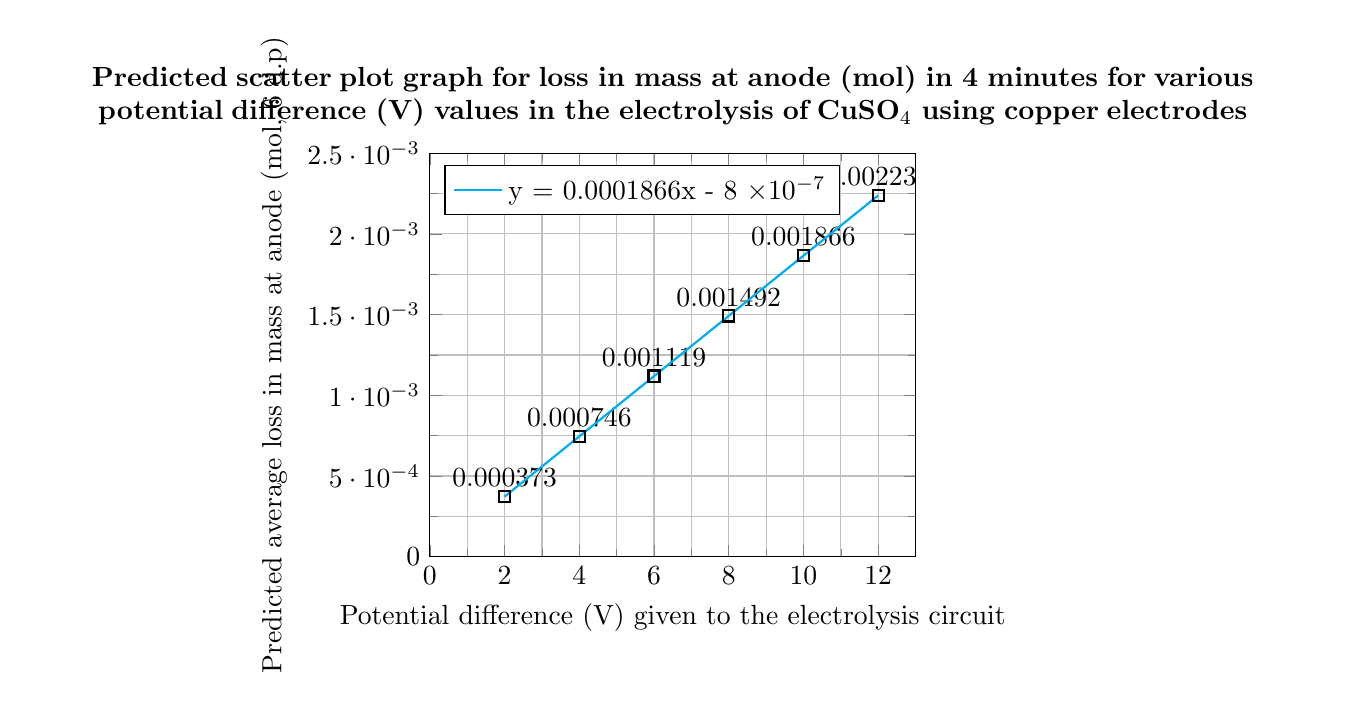
\begin{tikzpicture}
					\begin{axis}[scale=0.9,
   					title={\textbf{Predicted scatter plot graph for loss in mass at anode (mol) in 4 minutes for various potential difference (V) values in the electrolysis of CuSO$_{4}$ using copper electrodes}},
   					title style={align=center, text width = 16.15cm},
  					xlabel={Potential difference (V) given to the electrolysis circuit},
  					ylabel={Predicted average loss in mass at anode (mol, 6 d.p)},
  					ylabel near ticks,
    				xmin=0, xmax=13,
    				ymin=0, ymax=0.0025,
    				xtick={0,2,4,6,8,10,12},
    				ytick={0,0.0005,0.001,0.0015,0.002,0.0025,0.003},
    				minor ytick={0,0.00025,0.0005,0.00075,0.001,0.00125,0.0015,0.00175,0.002,0.00225,0.0025,0.003},
    				minor xtick ={0, 1, 2, 3, 4, 5, 6, 7, 8, 9, 10, 11, 12},
    				legend pos=north west,
    				ymajorgrids=true,
    				xmajorgrids=true,
    				yminorgrids=true,
    				xminorgrids = true,
    				]

					\node [above] at (axis cs:  2,  0.000373) {$0.000373$};
					\node [above] at (axis cs:  4,  0.000746) {$0.000746$};
					\node [above] at (axis cs:  6,  0.001119) {$0.001119$};
					\node [above] at (axis cs:  8,  0.001492) {$0.001492$};
					\node [above] at (axis cs:  10,  0.001866) {$0.001866$};
					\node [above] at (axis cs:  12,  0.002239) {$0.002239$};
				
				\addplot+[no marks, cyan, thick, domain=2:12] {0.0001866 * x - 0.0000008};
				
				\addplot[color=black, only marks, thick, mark=square, mark options={fill=white}] 
    coordinates {
         % /32(h)
         (2, 0.000373)
         (4, 0.000746)
         (6, 0.001119)
         (8, 0.001492)
         (10, 0.001866)
         (12, 0.002239)
         
        }; 
					
    				\legend{y = 0.0001866x - 8 $\times$10$^{-7}$}
					\end{axis}
					\end{tikzpicture}
					\end{center}		
				\end{figure}			
				
		As it can be observed, I predict, based off of my research, that as the potential difference given to the electrolysis circuit increases, the loss in mass at the anode also increases as a result of an increase in the rate of the reaction. The predicted trend line is proportional and has a positive gradient of 0.0001866 or 1.866 $\times$ 10 $^{-4}$. This was calculated as follows:
		
		\begin{equation*}
			\begin{split}
				m &= \frac{0.002239-0.000373}{10}\\
				&= \frac{0.001866}{10}\\
				&=0.0001866 \ or \ 1.866 \times 10 ^{-4}
			\end{split}
		\end{equation*}
		
	\section{Hypothesis:}
		Based off of my research above, I hypothesis that as the potential difference given to the electrolysis circuit increases, the rate of the reaction will increase and hence the loss in mass at the anode will also increase. I believe, that as an increase in potential difference also increases current, there will be physically higher quantities of electrons flowing from the cathode to the anode and thereby, more electrons will be available for reduction to take place, thus increasing the rate of the reduction reactions. This would directly cause the rate of the oxidation reactions to increase, as more $SO_{4}^{2-}$ ions are created, hence increasing the number of copper atoms liberated from the anode and overall speeding up the entire reaction. This increase in the rate of the reaction would mean an increase in the rate at which the anode loses mass, which would result in a greater total loss in mass at the anode within the 4 minutes that the reaction will take place for. 
		
	\section{Methodology:}
		\subsection{Independent variable:}
			The potential difference of the electrolysis circuit, measured in volts. This acts as a quantitative method of manipulating current, as current cannot be manipulated directly from the given setup. We will be performing a total of 18 electrolysis Oxidation-Reduction (Redox) reactions with 6 different potential difference values of 2, 4, 6, 8, 10 and 12 Volts (V) for a total of 6 datasets, each with 3 trials. This manipulation of potential difference will be achieved by changing the potential difference of the circuit from the power source and performing the necessary trials on 1 Molar Aqueous Copper(II) Sulphate. Each dataset of 3 trials corresponds with each potential difference value. The current values for each potential difference value will be noted down using an ammeter connected to the power source.
			
		\subsection{Dependent variable:}
			The loss in mass of the anode for each trial, measured in number of moles. This dependent variable acts as a quantitative measure for the rate of the electrolysis redox reaction. This will be achieved by measuring the original mass of the anode prior to and following the electrolysis reaction and utilising these values in the following equation to calculate the loss in mass at the anode:
			
			\begin{equation}
				Loss \ in \ mass \ of \ anode \ (g) \ = \ Initial \ mass \ of \ anode \ (g) \ - \ Final \ mass \ of \ anode \ (g)
			\end{equation}
			
			The calculated value in grams will then be converted to moles using the following equation:
			
			\begin{equation}
				Loss \ in \ mass \ of \ anode \ (mol) \ = \frac{Loss \ in \ mass \ of \ anode \ (g)}{M_{r} \ (u)}
			\end{equation}
			
			where $M_{r}$ represents the relative formulaic mass of the molecule/atom discharged from solution, which in this case is Copper. Given that Copper has a relative formulaic mass of 63.55 (2 d.p) the equation can be rewritten as:
			
			\begin{equation}
				Loss \ in \ mass \ of \ anode \ (mol) \ = \frac{Loss \ in \ mass \ of \ anode \ (g)}{63.55 \ u}
			\end{equation}
			
			The mass of the copper electrodes will originally be measured to 4 d.p in grams.
			
			\bigbreak
			
			This variable was chosen as a measure of the rate of the electrolysis reaction over other variables, such as measuring the gain in mass at the cathode, as it was observed during initial trial runs, that the copper present on the cathode easily breaks off and falls into solution, hence making measurements difficult to take. The cathode would also have to be constantly sanded to be used, hence resulting in the choice to measure the loss in mass at the anode.
			
		\subsection{Controlled variables:}
			\begin{longtable}{|>{\centering\arraybackslash}m{4.5cm}|>{\centering\arraybackslash}m{10.5cm}|}
				\hline
				\textbf{Variable controlled:} & \textbf{How and why it will be controlled:}\\
				\hline
				\hline
				Type of electrodes used & This variable will be controlled as, changing the type of electrodes used completely changes the reactions that take place at the anode and the cathode. A change in reactions mean different products will be produced and changing whether the anode even loses mass, which would make measurements not possible. To keep this variable constant and to allow for the reaction to take place, Copper electrodes will be used.\\
				\hline
				Concentration of Copper sulphate solution & This variable will be controlled as changing the concentration of the Copper(II) Sulphate solution used in each trial changes the amount of Copper(II) Sulphate ions present in the electrolyte, thus affecting the rate of reaction. A change in the rate of reaction from trial to trial would mean the loss in mass at the anode would be affected by external factors, hence making all data invalid. Lowering the concentration significantly would also mean that due to the position of copper in the electrochemical series and the significantly higher number of hydrogen ions, the hydrogen may become preferentially discharged instead of copper, yielding no results in the experiment. To avoid this, the variable be kept constant by only using 1 M Copper(II) Sulphate solution for each trial.\\
				\hline
				Volume of Copper Sulphate solution used in each trial & Changing this variable also directly changes the amount of Copper(II) Sulphate ions present in the solution, meaning the rate of reaction will change and hence the loss in mass at the anode would also change, thus interfering with the data collected. In order to prevent invalid data, this will be kept constant by only using 100 mL of 1 M Copper(II) Sulphate solution in each trial.\\
				\hline
				Time duration of each trial & This will need to be kept constant as changing the time for which each trial runs will affect the loss in mass at the anode as not setting a limit on the time the reaction runs for changes the number of copper atoms oxidised and reduced significantly. Hence, the reaction will run for only 4 minutes for each trial.\\
				\hline
				Temperature of the environment in which the experiment takes place & Changing the temperature would directly influence the kinetic energy that each atom has, which changes the rate of reaction as the ions in solution move to the respective electrodes at a faster or slower rate, which directly affects the rate of the electrochemical reaction, hence the loss in mass at the anode will begin to vary. This will be kept constant by keeping the room temperature at 23$^{o}$C.\\
				\hline
				Pressure of the environment in which the experiment takes place & This variable will also be controlled as changing the pressure also has the same effect as changing the temperature, that is the ions reach the anode or cathode faster, hence the rate of reaction would be affected, which would change the loss in mass at the anode within the 4 minutes that each reaction runs for. This will be kept constant at relatively the same value (as we do not have absolute control over this value with equipments that we have access to).\\
				\hline
				Surface area of electrode submerged under the copper sulphate solution & This is kept constant as changing this value changes the area on which the ions can act on. Therefore, if more or less ions act on more or less atoms of the electrode, due to the larger or smaller surface area, the rate of the reaction will change, thereby also changing the mass lost at the anode at the end of the 4 minutes. Therefore, this is kept constant by maintaining the size of the copper electrode and the height of the clamps on the clamp stand from the base. This will ensure that the same surface area of the electrode is submerged for each trial.\\
				\hline 
				Thickness of copper electrodes & This is one of the separate values that is also kept constant as it is one of the values that can affect the surface area of the electrode, which can affect the rate of the reaction due to reasons described above. Hence, this is kept constant at 0.03 mm for all trials.\\
				\hline
				Type of current utilised & This is kept controlled as changing the current from D.C to A.C would mean the electrodes would begin to constantly switch between being the anode and the cathode, thereby not allowing the copper ions in solution to discharge and allow the reaction to proceed. To prevent this from being an issue and affecting the reaction, D.C current will be used throughout all trials,\\
				\hline 
				Distance between electrodes & Changing the distance between the electrodes changes the resistance of the electrolyte, hence changing the current flowing through it. When the electrodes are brought closer together, there is a lower resistance, resulting in an increased current flowing through, with the inverse occurring when the distance is increased. The changing current affects the rate of the reaction and thereby affects the loss in mass at the anode. Hence, this is kept constant by ensuring that the clamps are set to be 6 cm from the clamp join at the clamp stand for all trials.\\
				\hline
			\end{longtable}
		
		\subsection{Equipment and Diagrams:}
			\subsubsection{Materials list:}
				\begin{longtable}{|>{\centering\arraybackslash}m{5.5cm}|>{\centering\arraybackslash}m{9.5cm}|}
					\hline
					\textbf{Materials:} & \textbf{Quantity:}\\
					\hline
					\hline
					Clamp Stands & 2 stands\\
					\hline
					Clamps & 2 clamps\\
					\hline
					Power pack & 1 pack\\
					\hline
					Wires & 3 wires\\
					\hline
					Crocodile clips & 2 clips\\
					\hline
					0-5 A range Ammeter & 1 ammeter\\
					\hline
					0.04 cm thick Copper plate & 90 cm$^{2}$ area plate (measured on one side of plate)\\
					\hline
					1 M Copper sulphate solution & 110 mL \\
					\hline
					100 mL glass beaker & 1 beaker\\
					\hline
					Precise instruments to measure with & 1 piece \footnote{E.g. A pen or pencil}\\
					\hline
					Erasable instruments to measure with & 1 piece \footnote{E.g. A Whiteboard marker}\\
					\hline
					Instruments to record data collected on and with \footnote{E.g. A pen and paper} & 1 set\\
					\hline
					15 cm Ruler & 1 ruler\\
					\hline
					Tissue paper & 2 pieces (1 contingency)\\
					\hline
					Sandpaper (500 grit) & 5 cm $\times$ 5 cm piece\\
					\hline
					Scissors & 1 pair of scissors\\
					\hline
					Stopwatch & 1 stopwatch\\
					\hline
					Measuring cylinder (100 mL) & 1 cylinder\\
					\hline
					Funnel & 1 funnel\\
					\hline
					Filter paper & 1 paper disc of radius 5 cm\\
					\hline
					Pipette & 1 pipette\\
					\hline
					Safety glasses & Equal to number of individuals performing the experiment\\
					\hline
					Latex gloves & Equal to number of individuals performing the experiment\\
					\hline				
				\end{longtable}
				
			\subsubsection{Equipment setup:}
				\begin{figure}[H]
					\vspace{-4mm}
					\begin{center}
					\end{center}
					\caption{Equipment setup for electrolysis of 1 M Copper(II) Sulphate solution using copper electrodes investigation}
				\end{figure}
		\subsection{Experiment procedure:}
			The procedure below allows for sufficient relevant data to be gathered, as over 18 trials of data over a wide range of potential difference values are collected.
			
			\begin{enumerate}
				\item Cut the copper plate into copper electrodes of size 5 cm $\times$ 1 cm using the ruler, scissors and the precise measuring instrument.
				\item Place 2 clamp stands next to each other, ensuring the bases touch and create a flat surface and the stands are as far as possible in orientation from each other.
				\item Measure 9 cm from the base of the first clamp stand using the 15 cm ruler.
				\item Mark this point using the erasable instrument for measurement.
				\item Attach a clamp to this point, ensuring the point at which the clamp connects to the stand overlaps the mark made in the previous step.
				\item Adjust the protruding clamp to be 11 cm from the clamp joint.
				\item Repeat steps 3-6 for the second clamp stand.
				\item Connect the negative terminal of the power pack to the negative terminal of the ammeter using a wire.
				\item Connect a wire from the positive terminal of the ammeter to a crocodile clip.
				\item Connect a wire from the positive terminal of the power pack to a crocodile clip.
				\item Measure half of the cover over the lead connected to both crocodile clips and mark this with the erasable instrument.
				\item Rinse the pipette with approximately 1 mL of the 1 M Copper(II) Sulphate solution.
				\item Rinse the 100 mL measuring cylinder with approximately 4 mL of the 1 M Copper(II) Sulphate solution.
				\item Place a funnel on top of the measuring cylinder.
				\item Pour and measure 100 mL of the 1 M Copper(II) Sulphate solution into the 100 mL measuring cylinder, using the pipette for minute adjustments.
				\begin{enumerate}
					\item Ensure that the liquid is measured at eye level, to prevent any parallax errors.
				\end{enumerate}
				\item Rinse the beaker using the pipette with 5 mL of the 1 M Copper(II) Sulphate solution.
				\item Pour the measured amounts of the 1 M Copper(II) Sulphate solution into the beaker.
				\item Place the beaker underneath the end points of the clamp, over the point where the base of the clamp stands meet.
				\item Measure the mass of a copper electrode, that will be the cathode, using the electronic balance and ensure that the mass is within the range 0.4000-0.4500 g and record this value using the instruments to record data.
				\begin{enumerate}
					\item If the measured mass is above or below this range, collect and use another copper electrode of size 5 cm $\times$ 1 cm
				\end{enumerate}
				\item Connect the cathode to the crocodile clip connected to the negative terminal of the power pack.
				\item Repeat step 19 with another copper electrode that will be the anode.
				\item Connect the anode to the crocodile clip connected to the positive terminal of the power pack.
				\item Clamp the cathode and anode to the clamp stands closest to the respective terminal from the power pack, ensuring that the top of the clamp touches the mark on the cover of the lead of the wire.
				\item Connect the power pack to a power outlet and set the potential difference on the power pack to be 2 volts.
				\item Close the switch on the power pack and start the stopwatch as soon as the power pack has been switched on.
				\item Record the reading on the ammeter.
				\item Switch off the power pack as soon as 4 minutes has been reached on the stopwatch.
				\item Unclamp the anode and remove the anode from the crocodile clip.
				\item Dab the anode lightly on a paper towel, ensuring to remove all liquid and residue on the anode.
				\item Measure the mass of the anode on the electric balance and record this value.
				\item Repeat steps 21-30 for 2 more trials.
				\item Unclamp the cathode and remove the cathode from the crocodile clip.
				\item Sand the cathode down to approximately the original mass of the cathode, measuring the mass of the cathode if needed.
				\begin{enumerate}
					\item If the mass of the cathode is less than 0.0300 g of the original mass of the cathode or less than 0.4000 g, collect and use another copper electrode as the cathode of size 5 cm $\times$ 1 cm.
				\end{enumerate}
				\item Shape and place the filter paper onto the funnel on top of the measuring cylinder.
				\item Pour through and thoroughly sieve the Copper(II) Sulphate solution.
				\item Pour the Copper(II) Sulphate solution back into the beaker for the next dataset.
				\item Repeat steps 20-36 for each dataset, for the remaining potential difference values of 4, 6, 8, 10 and 12 V.
			\end{enumerate}
		\subsection{Safety procedures:}
			\begin{enumerate}
				\item Ensure to handle glassware with utmost care to prevent breakage and injury as a result of damaged glassware.
				
				\item Safety glasses should be worn throughout to prevent Copper(II) Sulphate from coming in contact with the eyes of those who are performing the experiment. This is especially dangerous as Copper(II) Sulphate is a severe eye irritant and can damage the eyes.
				
				\item For girls or boys with long hair, ensure that they are tied in order to prevent hair from coming in contact with materials used in the experiment.
				
				\item Those who perform the experiment may opt to wear latex gloves to prevent the Copper(II) Sulphate from coming in contact with the body when handling equipment, as Copper(II) Sulphate is toxic.
										
				\item Ensure that the Copper(II) Sulphate does not come into contact with any body part or clothing as it may stain or be ingested accidentally if not washed properly.
				
				\item Dispose of all items contaminated with the Copper(II) Sulphate solution in the appropriate manner, by handing them off to a waste management centre or following any other guidelines set out in the specific country.

				\item Ensure that those performing the experiments wash their hands following the experiment to prevent accidental ingestion, as Copper(II) Sulphate can severely irritate the gastrointestinal tract.
			\end{enumerate}
			

	\section{Results:}
		\subsection{Data tables:}
			\begin{center}
				\textit{``*" Indicates an evident trial anomaly not included in the final average calculation, unless all trials are anomalies}
			\end{center}
			\textbf{Table 1 shows raw data for initial and final mass values calculated from various trials:}
			\begin{figure}[H]
			\begin{table}[H]
				\vspace{-4mm}
				\begin{minipage}{\textwidth}
					\begin{adjustbox}{width= \textwidth, center=\textwidth}
						\centering
						\begin{tabular}{|>{\centering\arraybackslash}p{3cm}|>{\centering\arraybackslash}p{2.5cm}|>{\centering\arraybackslash}p{2.5cm}|>{\centering\arraybackslash}p{2.5cm}|>{\centering\arraybackslash}p{2.5cm}|>{\centering\arraybackslash}p{2.5cm}|>{\centering\arraybackslash}p{2.5cm}|}
							\hline
							\multicolumn{1}{|c|}{\multirow{3}{3cm}{\textbf{Potential difference (V)}}} & \multicolumn{6}{c|}{\textbf{Initial and final mass values of anode after 4 minutes (g, 4 d.p)}}\\
							\cline{2-7}
							& \multicolumn{2}{c|}{\underline{Trial 1}} & \multicolumn{2}{c|}{\underline{Trial 2}} & \multicolumn{2}{c|}{\underline{Trial 3}}\\
							\cline{2-7}
							 & Initial & Final & Initial & Final & Initial & Final\\
							\hline
							\hline
							2 & 0.4156 & 0.3940 & 0.4237 & 0.3998 & 0.4194 & 0.3961\\
							\hline
							4 & 0.4046 & 0.3675 & 0.4262	 & 0.3845 & 0.4192 & 0.3828\\
							\hline
							6 & 0.4291 & 0.3772 & 0.4435 & 0.3874 & 0.4048 & 0.3401\\
							\hline
							8 & 0.4488 & 0.3608 & 0.4326 & 0.3256 & 0.4373* & 0.3306*\\
							\hline
							10 & 0.4436 & 0.3337 & 0.4382 & 0.3125 & 0.4451 & 0.3182\\
							\hline
							12 & 0.4191* & 0.2572* & 0.4057* & 0.2006* & 0.4077* & 0.1952*\\
							\hline
						\end{tabular}
					\end{adjustbox}
				\end{minipage}
			\end{table}
			\caption{Initial and final mass of copper anode for 3 trials for potential difference values of 2, 4, 6, 8, 10 and 12 V, after 4 minutes of immersion in 100 mL of 1M Copper(II) Sulphate solution}
			\end{figure}	

			\textbf{Table 2 shows loss in mass of anode, calculated from Table 1 and average values for each dataset:}
			
			\begin{figure}[H]
			\begin{table}[H]
				\vspace{-4mm}
				\begin{minipage}{\textwidth}
					\begin{adjustbox}{width= \textwidth, center=\textwidth}
						\centering
						\begin{tabular}{|>{\centering\arraybackslash}p{3cm}|>{\centering\arraybackslash}p{3.75cm}|>{\centering\arraybackslash}p{3.75cm}|>{\centering\arraybackslash}p{3.75cm}|>{\centering\arraybackslash}p{3.75cm}|}
							\hline
							\multicolumn{1}{|c|}{\multirow{2}{3cm}{\textbf{Potential difference (V)}}} & \multicolumn{4}{c|}{\textbf{Loss in mass of anode after 4 minutes (g, 4 d.p)}}\\
							\cline{2-5}
							& \underline{Trial 1} & \underline{Trial 2} & \underline{Trial 3} & \underline{Average}\\
							\hline
							\hline
							2 & 0.0216 & 0.0239 & 0.0233 & 0.0229\\
							\hline
							4 & 0.0371 & 0.0417 & 0.0364 & 0.0384\\
							\hline
							6 & 0.0519 & 0.0561 & 0.0647 & 0.0576\\
							\hline
							8 & 0.0880 & 0.1070 & 0.1067* & 0.0975\\
							\hline
							10 & 0.1099 & 0.1257 & 0.1269 & 0.1208\\
							\hline
							12 & 0.1619* & 0.2051* & 0.2125* & 0.1932*\\
							\hline
						\end{tabular}
					\end{adjustbox}
				\end{minipage}
			\end{table}
			\caption{Loss in mass of copper anode for 3 trials and average, for potential difference values of 2, 4, 6, 8, 10 and 12 V, after 4 minutes of immersion in 100 mL of 1M Copper(II) Sulphate solution}
			\end{figure}
			
			\textbf{Table 3 shows the charge that passed through the electrolyte in 4 minutes (C), Average loss in mass at the anode in grams and moles for different potential difference values:}
 
			\begin{figure}[H]
			\begin{table}[H]
				\vspace{-4mm}
				\begin{minipage}{\textwidth}
					\begin{adjustbox}{width= \textwidth, center=\textwidth}
						\centering
						\begin{tabular}{|>{\centering\arraybackslash}p{3.6cm}|>{\centering\arraybackslash}p{3.6cm}|>{\centering\arraybackslash}p{3.6cm}|>{\centering\arraybackslash}p{3.6cm}|>{\centering\arraybackslash}p{3.6cm}|}
							\hline
							\textbf{Potential difference (V)} & \textbf{Charge passed through electrolyte (C)} & \textbf{Average loss in mass at anode (g, 4 d.p)} & \textbf{Average loss in mass at anode (mol, 6 d.p)} & \textbf{Predicted loss in mass at anode (mol)}\\
							\hline
							\hline
							2 & 72 & 0.0229 & 0.000361 & 0.000373\\
							\hline
							4 & 140 & 0.0384 & 0.000604 & 0.000746\\
							\hline
							6 & 216 & 0.0576 & 0.000906 & 0.001119\\
							\hline
							8 & 288 & 0.0975 & 0.001534 & 0.001492\\
							\hline
							10 & 360 & 0.1208 & 0.001901 & 0.001866\\
							\hline
							12 & 432 & 0.1932 & 0.00304* & 0.002239\\
							\hline
						\end{tabular}
					\end{adjustbox}
				\end{minipage}
			\end{table}
			\caption{Average loss in mass of copper anode in moles and grams, against potential difference values of 2, 4, 6, 8, 10 and 12 V, charge passed through electrolyte and predicted loss in mass at the anode in moles, after 4 minutes of immersion in 100 mL of 1M Copper(II) Sulphate solution}
			\end{figure}

		\subsection{Sample calculations:}
			\textbf{Sample calculation for loss in mass (g) of anode for trial 1 of 2 V potential difference dataset:}
			
			\begin{equation*}
				\begin{split}
					Loss \ in \ mass \ at \ anode \ for \ trial \ 1 \ of \ 2 \ V \ dataset \ (g) \ &= \ 0.4156 \ g \ - \ 0.3940 \ g\\
					&= \ 0.0216 \ g \ (4 \ d.p)
				\end{split}
			\end{equation*}
			
			\textbf{Sample calculation for average loss in mass (g) of anode for 2 V potential difference dataset:}
			
			\begin{equation*}
				\begin{split}
					Average \ loss \ in \ mass \ at \ anode \ (g) \ &= \ \frac{0.0216 \ g \ + \ 0.0239 \ g \ + \ 0.0233 \ g}{3 \ trials}\\
					&= \ \frac{0.0688 \ g}{3 \ trials}\\p
					&= \ 0.0229 \ g \ (4 \ d.p)
				\end{split}
			\end{equation*}
			
			\textbf{Sample calculation for charge passed through the electrolyte in 4 minutes (240 seconds) at a potential difference of 2 V, calculated using equation 5:}
			
			\begin{equation*}
				\begin{split}
					Charge \ passed \ through \ the \ electrolyte \ (C) \ &= \ 0.3 A \ \times \ 240 \ s \\
					&= \ 72 \ C
				\end{split}
			\end{equation*}
			
			\textbf{Sample calculation for average loss in mass at anode in moles for potential a potential difference of 2 V, using equation 11:}
			
			\begin{equation*}
				\begin{split}
					Average \ loss \ in \ mass \ at \ anode \ (mol) \ &= \ \frac{0.0229 \ g}{63.55 \ u}\\
					&= 0.000361 \ mol \ (6 \ d.p)
				\end{split}
			\end{equation*}

		\subsection{Graph:}
		
		\begin{figure}[H]
					\vspace{-4mm}
					\begin{center}
					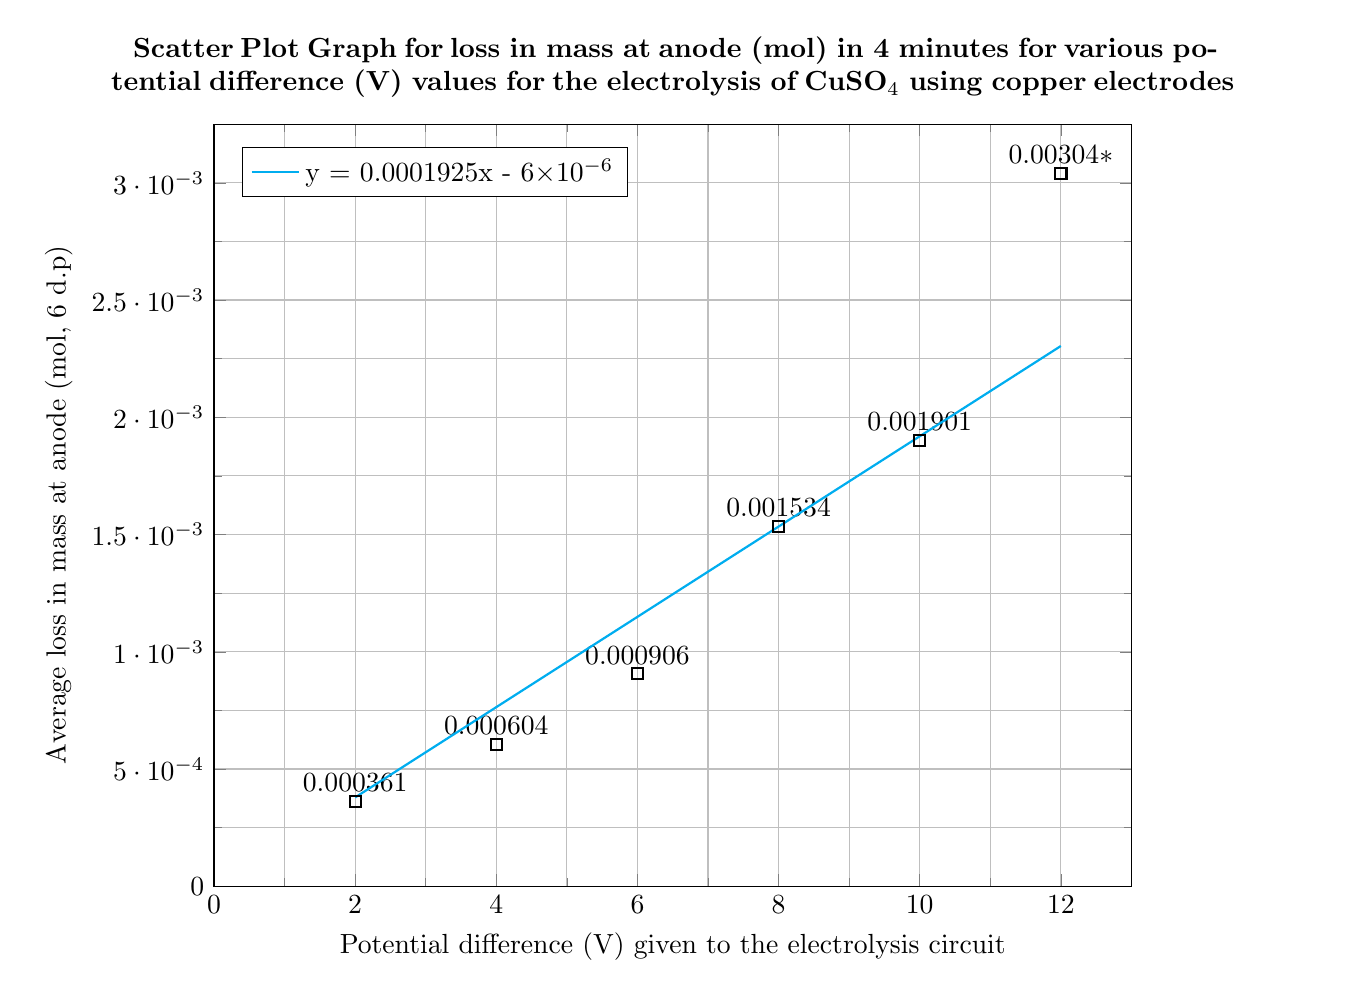
\begin{tikzpicture}
					\begin{axis}[scale=1.7,
   					title={\textbf{Scatter Plot Graph for loss in mass at anode (mol) in 4 minutes for various potential difference (V) values for the electrolysis of CuSO$_{4}$ using copper electrodes}},
   					title style={align=center, text width = 16.15cm},
  					xlabel={Potential difference (V) given to the electrolysis circuit},
  					ylabel={Average loss in mass at anode (mol, 6 d.p)},
  					ylabel near ticks,
    				xmin=0, xmax=13,
    				ymin=0, ymax=0.00325,
    				xtick={0,2,4,6,8,10,12},
    				ytick={0,0.0005,0.001,0.0015,0.002,0.0025,0.003},
    				minor ytick={0,0.00025,0.0005,0.00075,0.001,0.00125,0.0015,0.00175,0.002,0.00225,0.0025,0.00275,0.003,0.00325},
    				minor xtick ={0, 1, 2, 3, 4, 5, 6, 7, 8, 9, 10, 11, 12},
    				legend pos=north west,
    				ymajorgrids=true,
    				xmajorgrids=true,
    				yminorgrids=true,
    				xminorgrids=true,
    				]
					
					\node [above] at (axis cs:  2,  0.000361) {$0.000361$};
					\node [above] at (axis cs:  4,  0.000604) {$0.000604$};
					\node [above] at (axis cs:  6,  0.000906) {$0.000906$};
					\node [above] at (axis cs:  8,  0.001534) {$0.001534$};
					\node [above] at (axis cs:  10,  0.001901) {$0.001901$};
					\node [above] at (axis cs:  12,  0.00304) {$0.00304*$};
				
				\addplot+[no marks, cyan, thick, domain=2:12] { 0.0001925 * x -0.000006} ;
				\addplot[color=black,only marks,thick,mark=square, mark options={fill=white}] 
    coordinates {
         (2, 0.000361)
         (4, 0.000604)
         (6, 0.000906)
         (8, 0.001534)
         (10, 0.001901)
         (12, 0.00304)
         
        }; 	
				
    				\legend{y = 0.0001925x - 6$\times$10$^{-6}$}
					\end{axis}
					\end{tikzpicture}
					\end{center}		
					\caption{Scatter Plot Graph for loss in mass at anode (mol) in 4 minutes for various potential difference (V) values for the electrolysis of CuSO$_{4}$ using copper electrodes}
				\end{figure}	
		
	\section{Analysis:}
		\subsection{Trend present in data:}
			The graph above shows that the loss in mass at the anode (y-axis) is proportional to the potential difference given to the electrolysis circuit (x-axis). This is however not directly proportional as the trend line does not pass through the origin and as data was not collected for a potential difference value of 0. The graph, shows that as the potential difference given to the electrolysis circuit increases, the average loss in mass at the anode increases, signalling an increase in the rate of the electrolysis reaction, showing a positive correlation between these 2 variables. For example, the average loss in mass at the anode increases from 0.000373 mol to 0.000746 mol as the potential difference increases from 2 V to 4 V.The equation for this graph is:
			
			\begin{equation}
				y = 0.0001925x - 6 \times 10^{-6}
			\end{equation}
			
			This equation is also included on the graph. However, the gradient calculations were not included on the graph for the sake of clarity. The gradient was calculated as follows:
			
			\begin{equation*}
			 	\begin{split}
			 		m &= \frac{0.001901-0.000361}{10-2}\\
			 		&= \frac{0.00154}{8}\\
			 		&= 0.0001925
			 	\end{split}
			\end{equation*}
			
			The trend for the data was calculated with the exclusion of the data collected for the potential difference value of 12 due to significant anomalies in the collection of data.
			
		\subsection{Scientific reasoning:}
			It can be interpreted from the graph and data table, that the reasoning for this relation between the independent and dependent variables could be that as the potential difference increases, the rate of the electrolysis reaction has seemed to increase, which would explain the direct increase in the loss of mass at the anode. This is because, a change in voltage affects the current flowing through the electrolyte, which would alter the physical number of electrons flowing through the electrolyte and available for use in reduction/oxidation. This affects the number and rate at which these oxidation reduction reactions take place, and thereby, increase the loss in mass at the anode. The magnitude of this change in the rate of the reaction increases with an increase in potential difference, as this increases current, which is clearly observed in the data collected. We can also observe however, that the this pattern is not completely portrayed, due to an anomaly with the data collected for the potential difference of 12 V, which is discussed below. However, the general trend is still well observable with the trend line and can be backed by scientific reasoning inferred from the data. The loss in mass at the anode evidently occured due to equations 7 and 8 and was observed on the electrodes:
			
			\begin{figure}[H]
				\vspace{-2mm}
				\begin{center}
				\end{center}
				\caption{Copper electrodes used in trial 1 of the 12 V dataset following the reaction. On the left is the anode and right is the cathode.}
			\end{figure}
			
		\subsection{Anomalies:}
			There were 2 significant anomalies in the data collected at trial 3 of the dataset for 8 V and the data collected for the dataset of 12 V. As it can be observed in the graph, the average loss in mass at the anode for the potential difference of 12 V is significantly different than the data collected for the potential difference values from 2 up till 10. However, I believe I have identified the causes of this anomaly and this is explored further in the evaluation section. However, the brief explanation is that we did not control the temperature of the solution directly and the electrode was breaking off in chunks, leaving significant bits behind in the solution. This was a fatal error that I failed to take into consideration, as even if I kept the temperature of the room constant, the direct temperature of the reaction was not being controlled, resulting in the data collected that I recognised to be anomalous only after calculating averages and comparing with the other average values. The other anomaly with trial 3 of the dataset for 8 V was due to human error, where my hands shook significantly when removing the electrode from the solution, due to which a chunk had broke off and due to the lack of access to more copper electrodes, the data collected was left to be anomalous and is further discussed in the evaluation section. All data values were compared to the ideal values predicted from equation 6 and were determined to be anomalies or not.
			
		\subsection{Alignment with hypothesis:}
			The data collected aligns with my hypothesis very closely. I had hypothesised that as the potential difference increased, the loss in mass would increase, which is evidently what was observed. All collected data values are within $\pm$ 0.00025 mol of the predicted value, with the exception of the anomalies. This yielded a very close representation of my predicted graph in the actual graph for the data collected. For example, the actual data collected for the loss in mass at the anode for 2 V was 0.000361 mol, compared to the predicted value of 0.000373 mol. This positive linear regression relationship also shows that my data agrees with the scientific reasoning of my hypothesis and can clearly be inferred from and supported by the collected data.
			
	\section{Evaluation:}
		\subsection{Validity of hypothesis:}
			I believe that the cause of the small deviations from the predicted values for the various collected loss in mass values was due to the lack of control over temperature. It can be observed that at 2 V, the loss in mass was extremely close to the predicted value, however, as the experiment progressed to higher potential difference values the deviation from the predicted values increased significantly. This would be caused by the increasing temperature of the electrolyte, as an increase in the current would mean increased collisions between the electrons and the molecules of the electrolyte, resulting in an increase in the temperature of the electrolyte. This increased temperature would cause an increase in the kinetic energy imparted to the molecules of the electrolyte, which translates to an increase in the rate of the reaction, and thereby the mass lost at the anode. Gaining a better control over temperature, using methods described in 6.2, would improve the validity of my data to suit my hypothesis. The concentration of the solution was also relatively low and could be increased to observe more significant effects and collect data that aligns closer to my predicted values. However, considering that the data presents a construable, quantitative trend that supports my hypothesis clearly, it can be observed that my hypothesis is valid. 
			\newpage
		\subsection{Validity and improvements to the method:}
			\begin{small}
				\begin{longtable}{|m{3.5cm}|m{7cm}|m{4.7cm}|}
					
					\hline
					
					\textbf{What went or could have gone wrong?} & \textbf{How did it affect my results?} & \textbf{How can this be improved upon?}\\
					
					\hline
					\hline
					
					The temperature of the electrolyte varied throughout the experiment and was not explicitly controlled in the controlled variables & 
					This had impacted the data I had collected, especially for the dataset of pH 12, severely. It became anomalous, could not be considered in the trend line and made inferring the data much more difficult. When conducting the experiment, we did not use instruments such as a thermometer to measure and ensure that the temperature of the electrolyte remained constant. Although the temperature of the room was constant, the electrolyte increased in temperature, which I had observed, especially during the collection of data for the potential difference of 12. The electrolyte heated up significantly and hence the rate of the reaction must have sped up quite greatly, thus making the measured value for the loss of mass of the anode significantly greater than the predicted values. Although in my controlled variables I had controlled the temperature of the room in which the experiment took place, I had not considered that the actual temperature of the electrolyte would vary, as we had only performed 6 pre-trial runs, each corresponding to a single run for each potential difference value, to collect data on the current readings. When performing these pre-trials, no heating effect was observed, however in the actual trial runs, this effect was observed. This issue even render all the data collected invalid, although unlikely, considering that the data exhibits a clearly observable trend line that correlates closely with the predicted ideal values. &
					The temperature of the \underline{electrolyte} is the factor that affects the rate of reaction of this reaction, not the temperature of the surrounding environment, hence this variable should have been controlled directly, rather than controlling it indirectly, via the volume of celery solution used. This can be achieved by using a thermometer to measure the temperature of the electrolysis setup and allowing the electrolyte to cool down or be replaced with a fresh amount after each trial. If heating during the trial is the cause and not residual heat from previous trials, an ice bath may be used to regulate the temperature of the setup. By keeping the temperature the same, the rate of the reaction would not be significantly affected.\\
					
					\hline
					
					The method caused the electrode to consistently break off, instead of eroding, especially at the higher potential difference values &
					This was also a major issue as I observed chunks of the electrode that were not eroded, break off when being removed for the purpose of measuring the mass. When this happened, the measured weight was significantly lower than what it should have been and was one of the other reasons I believe the data collected for the potential difference value of 12 V was anomalous. It was rather difficult to extract the broken off chunks of the electrode to measure their mass and hence, the final mass of the electrode was significantly smaller. The broken off chunks also affect the rate of the reaction for other trials that have these chunks present in the electrolyte as these chunks of previous electrodes become a part of the reaction. &
					This can be very simply resolved by using larger electrodes overall or increasing their thickness for all trials. This would resolve the issue and ensure that the data remains consistent as a larger electrode or a thicker electrode will have a higher resistance to creating breaking points and are more resistant to breaking at lower potential difference values. A purer electrode may also be used to prevent impurities from creating breaking points for the electrode to "flake off" from.\\
					
					\hline
					
					The method only called for 3 trials, while the common number of trials performed is usually 5 trials &
					A great improvement to the method to improve its accuracy in the collection of data, is to increase the number of trials performed. In the case of the anomalous result in the third trial for the dataset of 8 V, the average was taken over only 2 trials, which is rather inaccurate. Doing only 3 trials means my average was more inaccurate than doing 5 trials and is more susceptible to being influenced by errors. &
					This can be very simply resolved by ensuring that we gather more trials for each dataset. An optimal number of trials would be 5 for each dataset, as this can ensure that the data collected can remain accurate even with 1 or 2 anomalies. This also ensures that the data collected is less susceptible to errors.\\
					
					\hline
					
					The method did not consider that the orientation of the electrode could change when attached to the clamp &
					This was not a major issue, but occurred every once in a while. This was when the electrode was skewed when attached to the crocodile clip and during electrolysis. This would change the surface area of the electrode submerged under the electrode and thus would possibly affect the rate of the reaction, thus changing the loss in mass at the anode. However, this issue did not significantly affect the trend or data collected, but would be something to add to the method. &
					This can be simply fixed by pulling the clamp up from the clamp stand, clamping the electrode and attaching the clamp once again to the stand, instead of trying to squeeze our fingers in-between the clamp to clamp the electrodes and in the process changing their orientation and requiring re-clamping.\\
					
					\hline
				\end{longtable}
			\end{small}
		\subsection{Extensions to the investigation:}
			\begin{small}
				\begin{longtable}{|>{\centering\arraybackslash}m{5.2cm}|>{\centering\arraybackslash}m{10cm}|}
					\hline
					\textbf{What could be added to the benefit of the experiment?} & \textbf{How would this be accomplishes and what would this provide to the experiment?}\\
					\hline
					\hline
					Experimenting with other electrolytes &
					We could perform this experiment with various other electrolytes, such as aqueous Sodium Chloride, Lead(II) Bromide or even water, to observe how the rate of the electrochemical reactions change with different electrolytes and look at the different products produced and learn how to measure different products in different states, such as measuring a gas. This would not only provide a greater range of data but would allow for a deeper understanding into the half equations of different electrolytes and understand intuitively the reactions that take place in different electrolytes. A good candidate for this extension would be performing electrolysis with aqueous 1M Sodium Chloride.\\
					\hline
					Experimenting with other electrodes &
					We could look at using different electrodes and observe how the reaction changes. This would provide a greater insight into how the reaction can be influenced by using a specific electrode and it would also allow us to investigate the properties of these electrodes that cause such effects. This would allow us to understand the real world relevance of such electrodes and how and why they are used in different processes. For example, we could research into using graphite in the electrolysis of 1M Copper(II) Sulphate, and why simply using graphite electrodes yields entirely different products.\\
					\hline
					Experimenting with changes in other factors which affect the rate of reaction of electrolysis	 reactions, such as temperature, concentration of electrolyte, time the reaction is run for etc. &
					We could compare how changing the concentration of the electrolyte affects the rate of the reaction. This could look at changing another factor, such as one of those mentioned on the left and seeing the effect that this has on the rate of the reaction. This would allow us to look at how other factors yield different amounts and possibly even different products altogether and why this occurs at a molecular level.\\
					\hline
					Experimenting with electroplating &
					We could look at using this reaction to electroplate something and observe what factors affect the quality and speed at which the object is plated. We can achieve this in the case of 1M Copper(II) Sulphate by replacing the cathode with a conducting object that we aim to electroplate. We can manipulate the current and potential difference values to observe the specific changes in the quality or speed of the electroplating reaction.\\
					\hline
				\end{longtable}
			\end{small}
	\section{Conclusion:}
		Overall, our results show that as the potential difference given to the circuit increases, the rate of the reaction increases proportionally, which can be observed as proportional increase in the loss in the mass of the anode. This creates a positive correlation, with a trend line that has a positive gradient of 0.0001925. This has proven my hypothesis, with data collected being within a range of $\pm$ 0.00025 of the predicted values. To answer our research question - the relation between potential difference and the loss in mass at the electrode is that as potential difference increases, the loss in mass at the electrode increases proportionally as well and is a function of $y = 0.0001925x - 6\times 10^{-6}$.
	
	\section{Relation to statement of inquiry:}
		This investigation heavily relates to the statement of inquiry, as this scientific investigation allows us to look at how changing, in essence, the number of electrons that pass through the electrolyte affect the chemical interactions between the electrolyte and the electrodes. Here, we are attempting to understand this by observing the patterns created by such a reaction and attempting to understand how this affects our dependent variable (loss of mass at the anode, as a quantitative measure for the rate of the reaction). Here we are collecting data and observing patterns in order to construe the relationship between these variables. Here we are also able to observe how the product precipitated changes as the material of the electrode changes. Overall, this experiment has helped us understand how chemical bonds and interactions vary as elements of the setup vary and how this can be observed with the collection of quantitative data in the form of the loss in mass at the anode.

	\newpage
	\section{Bibliography:}
		\begin{center}
		\end{center} 
	
	
\end{document}